\documentclass[a4paper,11pt]{article}
\usepackage{amsmath}
\usepackage{wrapfig}
\usepackage{fancyhdr}
\usepackage{graphicx}
\usepackage{url}
\usepackage{float}
\usepackage{amsmath}
\usepackage{amssymb}
\usepackage[margin=1in]{geometry}

%\setlength{\voffset}{-0.5in}
%\setlength{\headsep}{5pt}
\newcommand{\suchthat}{\;\ifnum\currentgrouptype=16 \middle\fi|\;}


%===========---------================
% Author John H Allard
% CMPE 12, Lab #2 Write-up
% October 9th, 2014
%===========---------================


\title{ CMPE 12 Lab Report \# 2 \\[7 in]}
\author{John Allard \\ TUTOR \\ Lab Section \#2}
\date{October 16th, 2014}

\begin{document}
\maketitle
\newpage
\tableofcontents
\newpage

%*************************************%
%************* OVERVIEW **************%
%*************************************%

\section{Overview}
This lab, unlike lab \#1, consisted of a single goal. Construct a simple 8-bit ALU using the MultiMedia Logic program. The entire ALU had to be built from scratch, minus a few hints on how to design the input and output layout for the device. This meant that it was completely up to us to determine how we want to divide up, layout, and implement the functionality required by this lab. This also implied that a large portion of our time would be spent planning and prototyping the different parts of the ALU individually before assembling them into one complete unit. \par
Relative to modern ALU's, the one developed in this lab will be a quite simple one. Our ALU is only required to provide two logic functions (AND, NOT), and an ADD function. It would be useful to also include other logic functions like OR, XOR, or NAND, but technically all of these functions can be constructed out of numerous NOT and AND calls, so our ALU is complete. It would also be nice if it could operate on more than 8-bit inputs, but the wiring for a 32-bit or even 16-bit ALU would be much too cumbersome to reasonably accomplish in a bulky simulator like MML. \par  Because this device consists of so many individual components, it has been laid out over 6 consectutive pages in the \texttt{lab2.lgi} document. The list below will inform you what components are on which pages :
\begin{enumerate}
\item Page 1 - Opcode input, operand inputs, input and output displays, state LED's.
\item Page 2 - Source Registers 1 and 2 (SR1 \& SR2), Instruction Register (IR), and first level Opcode decoder.
\item Page 3 - 8-bit Ripple Carry Full-Adder. This takes the data from the SR1 and SR2 registers, the carry-in bit, and produces an 8-bit sum plus a carry out bit.
\item Page 4 - Destination Register (DR), holds the final output of the last operation. This page also contains the logic that controls the output LEDs (P, N, Z, COUT, etc.).
\item Page 5 - ALU Logic Control Section. This section takes the data from SR1 and SR2 and performs the AND and NOT operations on the data. 
\item Page 6 - The final output destination multiplexer. This device takes the results from all of the ALU's functions (AND, ADD, NOT), and determines which of these outputs to route to the destination register (DR) based on the current instruction from the IR. 
\end{enumerate}

When you are simulating my ALU, you will pretty much only need to be looking at the first page. This page contains everything needed to set the inputs and read the outputs. The other 5 pages consist of the underlying circuitry, which will be described in the following 5 or 6 sections of this paper.

%*************************************%
%*********** INPUT/OUTPUT ************%
%*************************************%
\section{Device IO}
This project obviously needs some sort of input and output section to allow the user to properly interact with the ALU. All of the IO components can be found on the first page of the \texttt{lab2.lgi} document, and the layout will look pretty similar to the one presented to us in \texttt{Figure 4} of \texttt{the Lab 2 Instructions PDF}. A high level description of how the user interacts with the ALU is as follows :
\begin{enumerate}
\item Choose an instruction by entering an opcode. 
\item Based on the opcode entered, enter either one or two 8-bit inputs via the HEX keypads. 
\item If needed, set the carry-in bit (only does something during an ADD instruction).
\item Press the `CLOCK' button. 
\item Your output should not be displayed on the output display and the state LEDs should be lit or dim appropriately.
\item Either press the reset button, or go back to the top of this list.
\end{enumerate}

A more in-depth description of the ALLU IO functionality can be found in the two subsections below.

 %\begin{figure}[h!]
  \begin{wrapfigure}{l}{0.72\textwidth}
     %\centering
       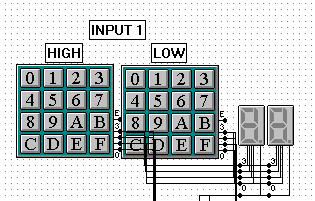
\includegraphics[width=4in]{pictures/8bitinput}
     \caption{8-bit Input Device}
     \label{fig:8bitinput}
  \end{wrapfigure} 

\subsection{Input}
The input for the ALU is relatively simple, and is analagous to many other operations in programming. You need to choose a function to perform, and then give this function some agruments. This function will return a resul that depends on the arguments provided. This is almost exactly how the ALU that I built works, where in our case we have 3 function choices and two input choices. Below is a description of every input that the ALU needs.

   \begin{wrapfigure}{l}{0.72\textwidth}
     %\centering
       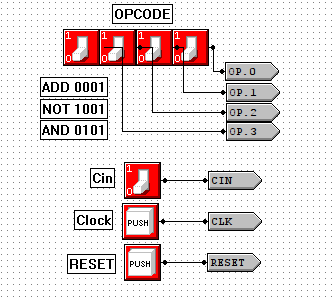
\includegraphics[width=4in]{pictures/opcodeinput}
     \caption{Opcode Input Section}
     \label{fig:opcodeinput}
  \end{wrapfigure} 

  \begin{itemize}
  \item \textbf{One or Two 8-bit Numbers -} These are the two possible arguments that can be used by any function the ALU completes. Both of these inputs are 8-bit numbers, but they individually are entered as a 2-digit HEX number. These numbers are signed using the two's compliment method, so any HIGH hex digit above 7 will have a leading one which will make the number negative. The input for each of these two 8-bit numbers is shown in Figure \ref{fig:8bitinput}

  \item \textbf{4-bit OpCode -} The ALU needs to know which function to perform. Although a 4-bit opcode input could technically specify 16 unique instructions to the ALU, we will only be using three of the available values ( $[1001], [0001], [0101]$ for NOT, ADD, and AND respectively). The opcode is entered by setting 4 switches to either a high or low state, as seen in Figure \ref{fig:opcodeinput}.

  \item \textbf{Carry-In, Clock, and Reset -} The carry-in bit only does something when you also enter the ADD opcode, in this case is sets the carry-in bit to high for the 8-bit full adder. The Clock button allows you to simulate a single clock cycle for the ALU. If you've just set an opcode and an input, you would need to press the clock button to have the inputs propogate through the ALU causing it to generate the correct output. Finally, the reset button just sets all of the memory in the ALU to \texttt{0}.

  \end{itemize}
 \subsection{Output}

  The output for the ALU is also extremely simple, it consists of 2 display screens (one for each HEX digit) and a handful of LED's that give the user more information on the current state of the ALU. The output displays will look identical to the input displays, except they will be labeled output and won't be connected to any keypads. After you complete an operation, the output will be displayed here. If you entered an invalid opcode, you will see an output of \texttt{BC}, which stands for `bad (op)code'. Refer to the previous section for the valid input opcodes. The LED array will tell the user various information about the state of the ALU, for more information, see Figure \ref{fig:resultinfo}

      \begin{wrapfigure}{l}{0.72\textwidth}
     %\centering
       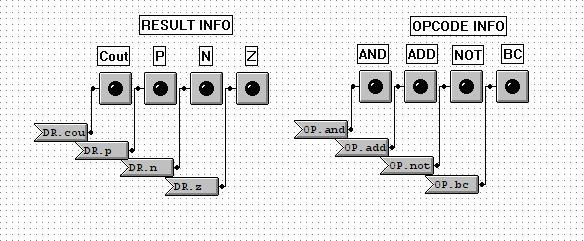
\includegraphics[width=5in]{pictures/resultinfo}
     \caption{LED Output Display}
     \label{fig:resultinfo}
  \end{wrapfigure} 
%*************************************%
%************* REGISTERS *************%
%*************************************%
\section{Registers}

\subsection{Source Registers}

\subsection{Instruction Register}

\subsection{Destination Register}

%*************************************%
%*************** LOGIC ***************%
%*************************************%
\section{ALU Logic}

\subsection{NOT}

\subsection{AND}

%*************************************%
%************* Arithmetic ************%
%*************************************%
\section{ALU Arithmetic}


%*************************************%
%*********** DATA SELECTION **********%
%*************************************%
\section{Output Selection}

\subsection{Bad Code}
%*************************************%
%************** ANALYSIS *************%
%*************************************%



\end{document}